\documentclass[conference]{IEEEtran}
% Build: python scripts/make_paper_tables.py && cd docs/paper && tectonic paper.tex   (or: make paper)

\usepackage[T1]{fontenc}
\usepackage{newtxtext,newtxmath}        % Times, as IEEEtran expects (works under XeTeX/Tectonic)
\usepackage{amsmath}
\usepackage{graphicx}
\usepackage{booktabs}
\usepackage{cite}
\usepackage{url}
\usepackage[hidelinks]{hyperref}

\graphicspath{{../figures/}}
\newcommand{\XgbMAEFifteen}{3.02}
\newcommand{\XgbMAEThirty}{3.51}
\newcommand{\XgbMAESixty}{4.01}
\newcommand{\LstmMAEFifteen}{2.97}
\newcommand{\LstmMAEThirty}{3.55}
\newcommand{\LstmMAESixty}{4.35}
\newcommand{\StgatMAEFifteen}{2.84}
\newcommand{\StgatMAEThirty}{3.32}
\newcommand{\StgatMAESixty}{3.95}
\newcommand{\DcrnnMAEFifteen}{2.64}
\newcommand{\DcrnnMAEThirty}{3.05}
\newcommand{\DcrnnMAESixty}{3.57}
\newcommand{\XgbNbMAEFifteen}{2.91}
\newcommand{\XgbNbMAEThirty}{3.42}
\newcommand{\XgbNbMAESixty}{3.95}
\newcommand{\PersistMAEFifteen}{3.49}
\newcommand{\PersistMAEThirty}{4.20}
\newcommand{\PersistMAESixty}{5.37}
\newcommand{\HybridMAEFifteen}{2.62}
\newcommand{\HybridMAEThirty}{3.01}
\newcommand{\HybridMAESixty}{3.47}
\newcommand{\DcrnnGainFifteen}{12.3}
\newcommand{\DcrnnGainThirty}{13.1}
\newcommand{\DcrnnGainSixty}{11.0}
\newcommand{\StgatGainFifteen}{5.8}
\newcommand{\StgatGainThirty}{5.4}
\newcommand{\StgatGainSixty}{1.3}
\newcommand{\HybridGainFifteen}{13.0}
\newcommand{\HybridGainThirty}{14.2}
\newcommand{\HybridGainSixty}{13.3}
\newcommand{\HybridOverDcrnnFifteen}{0.8}
\newcommand{\HybridOverDcrnnThirty}{1.2}
\newcommand{\HybridOverDcrnnSixty}{2.6}
\newcommand{\TestDays}{24}
\newcommand{\DcrnnMinDaysBetter}{24}
\newcommand{\StgatSixtyPBoot}{0.021}
\newcommand{\StgatSixtyPDm}{0.061}
\newcommand{\StgatSixtyDays}{16}
\newcommand{\AttDownNormal}{52.0}
\newcommand{\AttDownAhead}{62.5}
\newcommand{\AttSensors}{163}
\newcommand{\AttShifted}{149}
\newcommand{\DegGainLow}{4.3}
\newcommand{\DegGainHigh}{12.8}
\newcommand{\OnsetXgbFifteen}{16.2}
\newcommand{\OnsetXgbThirty}{20.1}
\newcommand{\OnsetXgbSixty}{19.1}
\newcommand{\OnsetDcrnnFifteen}{13.3}
\newcommand{\OnsetDcrnnThirty}{18.2}
\newcommand{\OnsetDcrnnSixty}{20.7}
\newcommand{\MapCongested}{103}
\newcommand{\MapXgbCaught}{75}
\newcommand{\MapGraphCaught}{88}
\newcommand{\MapSensorsBetter}{198}
\newcommand{\AblNoGraphSixty}{4.35}
\newcommand{\AblNoGraphDelta}{0.40}
\newcommand{\AblFwdSixty}{4.05}
\newcommand{\AblFwdDelta}{0.10}
\newcommand{\AblBwdSixty}{4.02}
\newcommand{\AblBwdDelta}{0.07}
\newcommand{\AblRandomSixty}{4.18}
\newcommand{\AblRandomDelta}{0.22}
\newcommand{\AblNoDropSixty}{3.92}
\newcommand{\AblNoDropDelta}{-0.03}
\newcommand{\AblDcrnnFwdSixty}{3.72}
\newcommand{\AblDcrnnFwdDelta}{0.15}
\newcommand{\AblDcrnnKoneSixty}{3.57}
\newcommand{\AblDcrnnKoneDelta}{0.00}
\newcommand{\XgbRMSESixty}{7.28}
\newcommand{\XgbNbRMSESixty}{7.14}
\newcommand{\DcrnnRMSESixty}{7.67}
\newcommand{\HybridRMSESixty}{7.30}
\newcommand{\NTests}{53}

% \input is not expandable inside tabular since LaTeX 2020; the TeX primitive is
\makeatletter\newcommand{\tabinput}[1]{\@@input #1 }\makeatother

\begin{document}

\title{Do Graph Neural Networks Close the Spatial Gap?\\
Leak-Free Traffic Speed Forecasting on METR-LA with Graph Attention, Diffusion and a Hybrid Tree Corrector}

\author{\IEEEauthorblockN{Team T036}
\IEEEauthorblockA{Newton School of Technology, Rishihood University\\
Code and results: \url{https://github.com/ManasSaxena14/TrafficFlowControl_AIML-DL_T036}}}

\maketitle

\begin{abstract}
We ask whether a model that reads the road network forecasts freeway speed better than strong models that look at one
sensor at a time, and where any gain comes from. On METR-LA (207 Los Angeles sensors, 5-minute speeds) we build a
leak-free protocol (chronological split with a purge gap, train-only scaling, masked outages), a ladder of six
per-sensor baselines whose best member is XGBoost, and four experiments that measure what such models miss. We then
train two graph neural networks on the same windows: a spatio-temporal graph attention network (STGAT) whose attention
runs over both directions of every road link, and a PyTorch port of the diffusion convolutional recurrent network
(DCRNN). DCRNN lowers test MAE against XGBoost by \DcrnnGainFifteen\%, \DcrnnGainThirty\% and \DcrnnGainSixty\% at 15,
30 and 60 minutes, on every one of the \TestDays{} test days; STGAT also improves on XGBoost, mostly at short horizons.
Ablations show the gain comes from the real road graph and from listening to downstream neighbours, and the trained
attention shifts downstream when a slowdown is approaching. Finally, a hybrid that corrects DCRNN with a small,
regularised gradient-boosted tree model, fitted on held-out data, lowers DCRNN's error by a further
\HybridOverDcrnnSixty\% at 60 minutes.
\end{abstract}

\begin{IEEEkeywords}
traffic forecasting, graph neural networks, graph attention, diffusion convolution, hybrid models, METR-LA
\end{IEEEkeywords}

\section{Introduction}
Short-term traffic speed forecasts feed route guidance and signal timing. A per-sensor model forecasts each road
segment from its own history; it cannot see a jam that is forming one link away. Graph neural networks (GNNs) read the
road network directly and are the standard approach on benchmarks such as METR-LA~\cite{li2018dcrnn,yu2018stgcn,
wu2019graphwavenet}. Reported gains, however, are usually measured against weak baselines, under window-level random
or overlapping splits, and as one average number.

This project tests the claim under a deliberately strict protocol and asks where the gain comes from. Our
contributions are:
\begin{itemize}
\item a leak-free pipeline with automated tests (chronological split with a purge gap, train-only scaling, outages
masked as missing rather than treated as 0~mph) shared by every model;
\item a strong baseline ladder and four measurements of the \emph{spatial gap} left by per-sensor models;
\item STGAT, a graph attention network with bidirectional, direction-aware edges motivated by measured upstream
propagation of congestion, and a faithful PyTorch DCRNN, both evaluated with 3 seeds and day-level significance tests;
\item ablations of graph, direction, hops and regularisation, and an inspection of what the attention learned;
\item a justified ML+DL hybrid: a regularised XGBoost residual corrector on top of DCRNN.
\end{itemize}

\section{Related Work}
\textbf{Classical and per-sensor models.} Historical averages, linear models and tree ensembles such as Random
Forest~\cite{breiman2001rf} and XGBoost~\cite{chen2016xgboost} forecast each location from engineered lags and calendar
features. Recurrent networks (LSTM~\cite{hochreiter1997lstm}, GRU~\cite{cho2014gru}) learn temporal patterns without
hand-made features, but still treat sensors independently.

\textbf{Graph-based forecasting.} Graph convolutions~\cite{kipf2017gcn} aggregate neighbours with fixed normalised
weights. DCRNN~\cite{li2018dcrnn} models traffic as diffusion on a directed graph, with forward and backward random
walks inside a GRU encoder-decoder, and introduced the METR-LA benchmark protocol. STGCN~\cite{yu2018stgcn} replaces
recurrence with convolutions; Graph WaveNet~\cite{wu2019graphwavenet} learns an adaptive adjacency.
Graph attention (GAT)~\cite{velickovic2018gat} learns feature-dependent neighbour weights; GATv2~\cite{brody2022gatv2}
fixes GAT's static ranking of neighbours. Attention-based traffic models include ASTGCN~\cite{guo2019astgcn} and
GMAN~\cite{zheng2020gman}.

\textbf{Hybrids and evaluation.} Stacked generalisation~\cite{wolpert1992stacking} trains a second-level model on
held-out predictions of first-level models; we use it to let trees correct a GNN. Leakage through overlapping windows
and preprocessing is a known source of optimistic results~\cite{kaufman2012leakage}. We compare forecasters with the
Diebold-Mariano test~\cite{diebold1995dm} and its small-sample correction~\cite{harvey1997hln}. Signal control is often
studied in simulators such as CityFlow~\cite{zhang2019cityflow}; METR-LA covers freeways without signals, so control is
outside the results reported here.

\section{Data and Leak-Free Protocol}
\textbf{Data.} METR-LA~\cite{jagadish2014bigdata,li2018dcrnn} holds 34,272 five-minute speed readings for 207 loop
detectors (1 March--27 June 2012) and a directed adjacency
\begin{equation}
W_{ij}=\exp\!\left(-d_{ij}^2/\sigma^2\right)\ \text{if}\ \ge 0.1,\ \text{else } 0,
\end{equation}
where $d_{ij}$ is the driving distance from sensor $i$ to $j$ (we rebuild it from raw distances and test it equals the
supplied matrix). 8.1\% of readings are 0~mph, which marks a sensor outage, not stopped traffic; 6.3 points of that are
whole-network outages. In the training period, congestion travels \emph{backwards}: on strongly coupled links the
downstream sensor slows first about four times as often as the upstream one, with an implied wave speed of about
16~km/h (Fig.~\ref{fig:prop}).

\textbf{Protocol.} Timestamps are split 70/10/20 chronologically; windows (12 steps in, 12 out) are cut inside each
block, so no target timestamp is shared between splits. Scaling and imputation statistics use training timestamps only.
Outages are NaN: inputs are forward-filled within the window (else the training slot mean) with a mask channel, and
targets are never imputed. Every model sees the same 60-minute history and is scored by the same masked MAE, RMSE and
MAPE in mph on the last 24 days. Peak hours are weekdays 07:00--09:59 and 16:00--19:59 on the predicted timestamp.

\begin{figure}[t]
\centering
\includegraphics[width=\columnwidth]{fig05d_propagation_example.png}
\caption{A jam reaches the downstream sensor first and the upstream sensor, 1.5~km back, 10 minutes later. A
per-sensor model at the upstream sensor cannot see it coming.}
\label{fig:prop}
\end{figure}

\section{Methods}
\subsection{Per-sensor baselines and the gap}
Six baselines share 46 features per sensor and time (12 speed lags, rolling statistics, recent change, missing flags,
cyclic time, segment statistics): persistence, historical average, ridge per sensor, a multi-output Random Forest,
XGBoost per horizon (the strongest, \XgbMAEFifteen/\XgbMAEThirty/\XgbMAESixty~mph at 15/30/60 min), and an LSTM with
weights shared across sensors. Four experiments measure the gap: error grows with horizon; XGBoost error is 5.9--6.4$\times$
larger in the 30 minutes after a congestion onset; residuals of linked sensors are correlated (0.20 one link apart,
0.00 for unconnected sensors); and adding hand-made neighbour speeds helps at every horizon, more from downstream than
upstream neighbours.

\subsection{STGAT: spatio-temporal graph attention}
A GRU with weights shared by all sensors encodes each sensor's 12 input steps into $h_i\in\mathbb{R}^{64}$. Two GATv2
layers~\cite{brody2022gatv2} then mix each sensor with its road neighbours:
\begin{align}
e_{ij}&=a^{\top}\,\mathrm{LeakyReLU}\!\left(W_r h_i+W_l h_j+W_e\,\epsilon_{ji}\right),\\
\alpha_{ij}&=\operatorname{softmax}_{j\in\mathcal{N}(i)} e_{ij},\qquad h_i'=\textstyle\sum_{j}\alpha_{ij}W_l h_j,
\end{align}
with 4 heads, residual connections and layer normalisation~\cite{ba2016layernorm}. Message passing on the raw matrix
would let a sensor hear only its upstream neighbours; since jams arrive from downstream, every link is added in both
directions with edge features $\epsilon=[W_{ij},\text{is\_reverse}]$, and attention learns how much each direction is
worth. A head maps $[h_i, h_i']$ to the 12 horizons as a change from the last speed. Our edge-list implementation runs on
CPU and Apple-silicon GPUs; a unit test shows it equals PyTorch Geometric's \texttt{GATv2Conv}. Mixing once after the
GRU, instead of at every input step, was 8$\times$ cheaper per batch, which made seeds and ablations affordable.

\subsection{DCRNN: diffusion convolutional recurrent network}
Following~\cite{li2018dcrnn}, the graph convolution is a $K$-step diffusion over forward and backward random walks,
\begin{equation}
X\star_{\mathcal G} f_\theta=\sum_{k=0}^{K-1}\left(\theta_{k,1}(D_O^{-1}W)^k+\theta_{k,2}(D_I^{-1}W^{\top})^k\right)X,
\end{equation}
which replaces every matrix product inside a GRU (DCGRU). A two-layer DCGRU encoder reads 12 steps and a decoder emits
12 steps with scheduled sampling~\cite{bengio2015scheduled}; $K=2$, 64 units, as in the reference configuration.

\subsection{Hybrid: graph model plus tree corrector}
DCRNN is the strongest model overall, while XGBoost with calendar and segment features remains better 60 minutes after
a congestion onset, and the two err differently. Following stacked generalisation~\cite{wolpert1992stacking}, the hybrid
keeps DCRNN as the backbone and learns its systematic error:
\begin{equation}
\hat y^{\text{hyb}}_{h}=\hat y^{\text{DCRNN}}_{h}+r_h\!\left(z,\ \hat y^{\text{DCRNN}}_{h},\ \hat y^{\text{XGB}}_{h}\right),
\end{equation}
where $r_h$ is a shallow XGBoost model (depth 3, $\ge$200 samples per leaf, L2 = 10, MAE objective) on compact inputs $z$
(current speed, recent change, time of day, weekend, free-flow speed). Because $r_h$ must see out-of-sample DCRNN
forecasts, it is fitted on the validation block (DCRNN only used it to choose its best epoch): the first 75\% of
validation windows fit $r_h$, the last 25\% decide its early stopping, and the test block is scored once.

\subsection{Training and regularisation}
All neural models minimise masked MAE in mph with Adam~\cite{kingma2015adam}, learning-rate drops ($\times0.1$ at epochs
20 and 30), gradient clipping at norm 5, and early stopping on validation MAE that never triggers before the last
learning-rate drop (at the initial DCRNN rate of 0.01, validation error is noisy). Regularisation: dropout
0.1~\cite{srivastava2014dropout} and layer normalisation in STGAT, scheduled sampling in DCRNN, each epoch drawn from a
fresh random half of the training windows, and a fixed graph (no learned adjacency). Main models use 3 seeds; ablations
use seed 0 with the main run's budget.

\subsection{Validation of the implementation}
\NTests{} automated tests guard the pipeline: chronological order and no shared target timestamps between splits,
train-only scaling, imputation that only looks back, masked targets contributing nothing to the loss, sensor order
matching the adjacency, the rebuilt adjacency equal to the supplied one, the attention layer equal to PyTorch Geometric's
\texttt{GATv2Conv}, information flowing only along the edges a model is given, diffusion directions, and the hybrid's
chronological fitting split. Regenerating the per-sensor baselines reproduces the previously reported numbers exactly.

\section{Results}
\subsection{Main comparison}
Table~\ref{tab:main} scores every model on the same test windows. DCRNN is best among single models at every horizon
(\DcrnnMAEFifteen/\DcrnnMAEThirty/\DcrnnMAESixty~mph). STGAT beats XGBoost by \StgatGainFifteen\% at 15 minutes but only
\StgatGainSixty\% at 60. The hybrid has the lowest MAE, MAPE and peak-hour MAE of all models
(\HybridMAEFifteen/\HybridMAEThirty/\HybridMAESixty~mph). RMSE tells a different story at 60 minutes: DCRNN
(\DcrnnRMSESixty) is above XGBoost (\XgbRMSESixty), because its rarer misses are larger, mostly when a jam starts; the
hybrid reduces this (\HybridRMSESixty) and XGBoost with neighbour features has the lowest RMSE (\XgbNbRMSESixty).
Fig.~\ref{fig:horizon} shows all 12 horizons.

\begin{table}[t]
\centering
\caption{Test MAE (mph) by horizon, 60-min RMSE, MAPE (\%) and weekday-peak MAE. $^{\dagger}$Mean of 3 seeds.}
\label{tab:main}
\setlength{\tabcolsep}{3.2pt}
\begin{tabular}{lrrrrrr}
\toprule
Model & 15 & 30 & 60 & RMSE & MAPE & Peak \\
\midrule
\tabinput{generated/tab_main.tex}
\bottomrule
\end{tabular}
\end{table}

\begin{figure}[t]
\centering
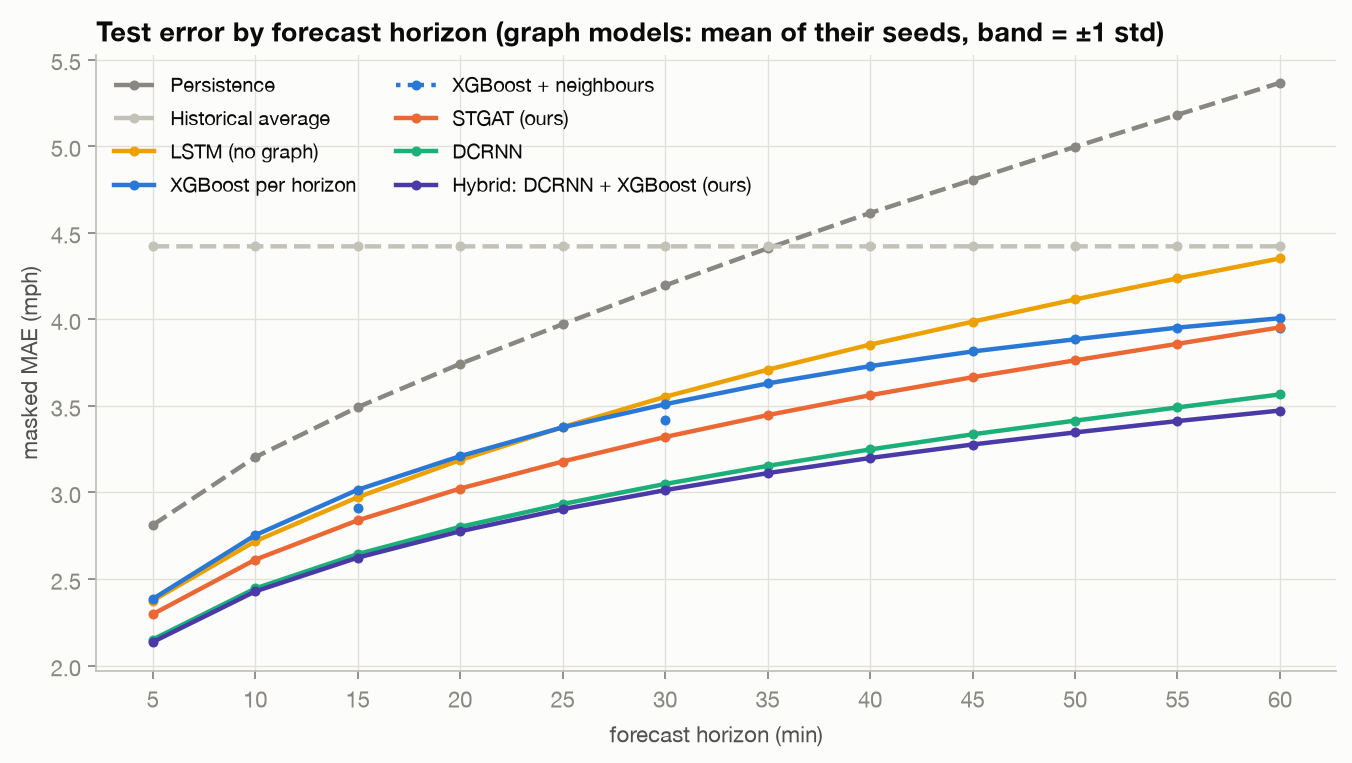
\includegraphics[width=\columnwidth]{fig15_final_error_by_horizon.png}
\caption{Test MAE by forecast horizon. Graph models: mean of 3 seeds, band = $\pm$1 std.}
\label{fig:horizon}
\end{figure}

\ifdefined\RefFifteen
\subsection{Reproducing the published DCRNN}
To check our port, we also train DCRNN under the reference protocol (windows split 70/10/20, scaler including outage
zeros). It reaches \RefFifteen/\RefThirty/\RefSixty~mph at 15/30/60 minutes, within \RefWorstPct\% of the published
2.67/3.08/3.56~\cite{li2018dcrnn}. Under our strict protocol the numbers are of the same size, so the stricter split
costs little but removes the shared target timestamps between splits.
\fi

\subsection{Significance}
Errors within a day are strongly correlated, so we aggregate them per test day and use a paired bootstrap over days
(10,000 resamples) and the Diebold-Mariano test~\cite{diebold1995dm,harvey1997hln}; each seed is tested and the worst is
reported (Table~\ref{tab:sig}). DCRNN is better than XGBoost on at least \DcrnnMinDaysBetter{} of \TestDays{} days at
every horizon. STGAT's 60-minute gain is weak (bootstrap $p$ = \StgatSixtyPBoot, DM $p$ = \StgatSixtyPDm).

\begin{table}[t]
\centering
\caption{Paired day-level tests (worst seed). Gain = MAE reduction vs the baseline.}
\label{tab:sig}
\setlength{\tabcolsep}{3.5pt}
\begin{tabular}{lrrrrr}
\toprule
Comparison & Min & Gain\% & Days & $p_{\text{boot}}$ & $p_{\text{DM}}$ \\
\midrule
\tabinput{generated/tab_sig.tex}
\bottomrule
\end{tabular}
\end{table}

\subsection{Ablations}
Table~\ref{tab:abl} varies one component at a time. Removing the graph (self-loops only) brings STGAT back to the
no-graph LSTM's level, so its gain comes from the neighbours. Keeping only downstream-to-upstream messages is better
than only upstream-to-downstream, and both directions are best, matching the measured backward propagation. The same
holds for DCRNN: without its backward random walk, its 60-minute MAE rises by \AblDcrnnFwdDelta~mph, while one diffusion
hop instead of two changes it by only \AblDcrnnKoneDelta~mph. A random
graph with the same number of links is clearly worse (+\AblRandomDelta~mph at 60 minutes), so the real road structure
matters, not just extra inputs. Removing dropout changes the 60-minute MAE by \AblNoDropDelta~mph: with 65k parameters
and 23k training windows STGAT does not overfit (its validation curve flattens without rising), so early stopping and
layer normalisation are enough. Regularisation matters where data is scarce: in the hybrid, an unregularised corrector
overfits (Section~\ref{sec:hybrid}).

\begin{table}[t]
\centering
\caption{Ablations: test MAE (mph), seed 0. $\Delta$ = change at 60 min vs the main run of the same model.}
\label{tab:abl}
\setlength{\tabcolsep}{3pt}
\begin{tabular}{lrrrr}
\toprule
Variant & 15 & 30 & 60 & $\Delta$60 \\
\midrule
\tabinput{generated/tab_ablation.tex}
\bottomrule
\end{tabular}
\end{table}

\subsection{The hybrid}\label{sec:hybrid}
Table~\ref{tab:hyb} compares hybrid designs on the same DCRNN seeds. A per-horizon blend helps a little; a residual
corrector on all 46 features overfits the short fitting block and is worse than DCRNN at 30 and 60 minutes; the
compact, regularised corrector improves DCRNN at every horizon, by \HybridOverDcrnnSixty\% at 60 minutes, where calendar
knowledge matters most.

\begin{table}[t]
\centering
\caption{Hybrid designs: test MAE (mph), mean $\pm$ std over DCRNN seeds.}
\label{tab:hyb}
\setlength{\tabcolsep}{3pt}
\begin{tabular}{lrrr}
\toprule
Design & 15 & 30 & 60 \\
\midrule
\tabinput{generated/tab_hybrid.tex}
\bottomrule
\end{tabular}
\end{table}

\subsection{Where the graph helps}
The gain of DCRNN over XGBoost at 60 minutes grows with connectivity, from \DegGainLow\% for sensors with 0--4 road links
to \DegGainHigh\% for sensors with 13 or more (Fig.~\ref{fig:where}). In the 30 minutes after a congestion onset, DCRNN's
15-minute error is \OnsetDcrnnFifteen{} versus \OnsetXgbFifteen~mph for XGBoost: it sees the slowdown at a neighbour first.
At 60 minutes ahead the jam has usually not started anywhere yet, and XGBoost's calendar knowledge is slightly better
(\OnsetXgbSixty{} vs \OnsetDcrnnSixty), the complementarity the hybrid exploits.

\begin{figure*}[t]
\centering
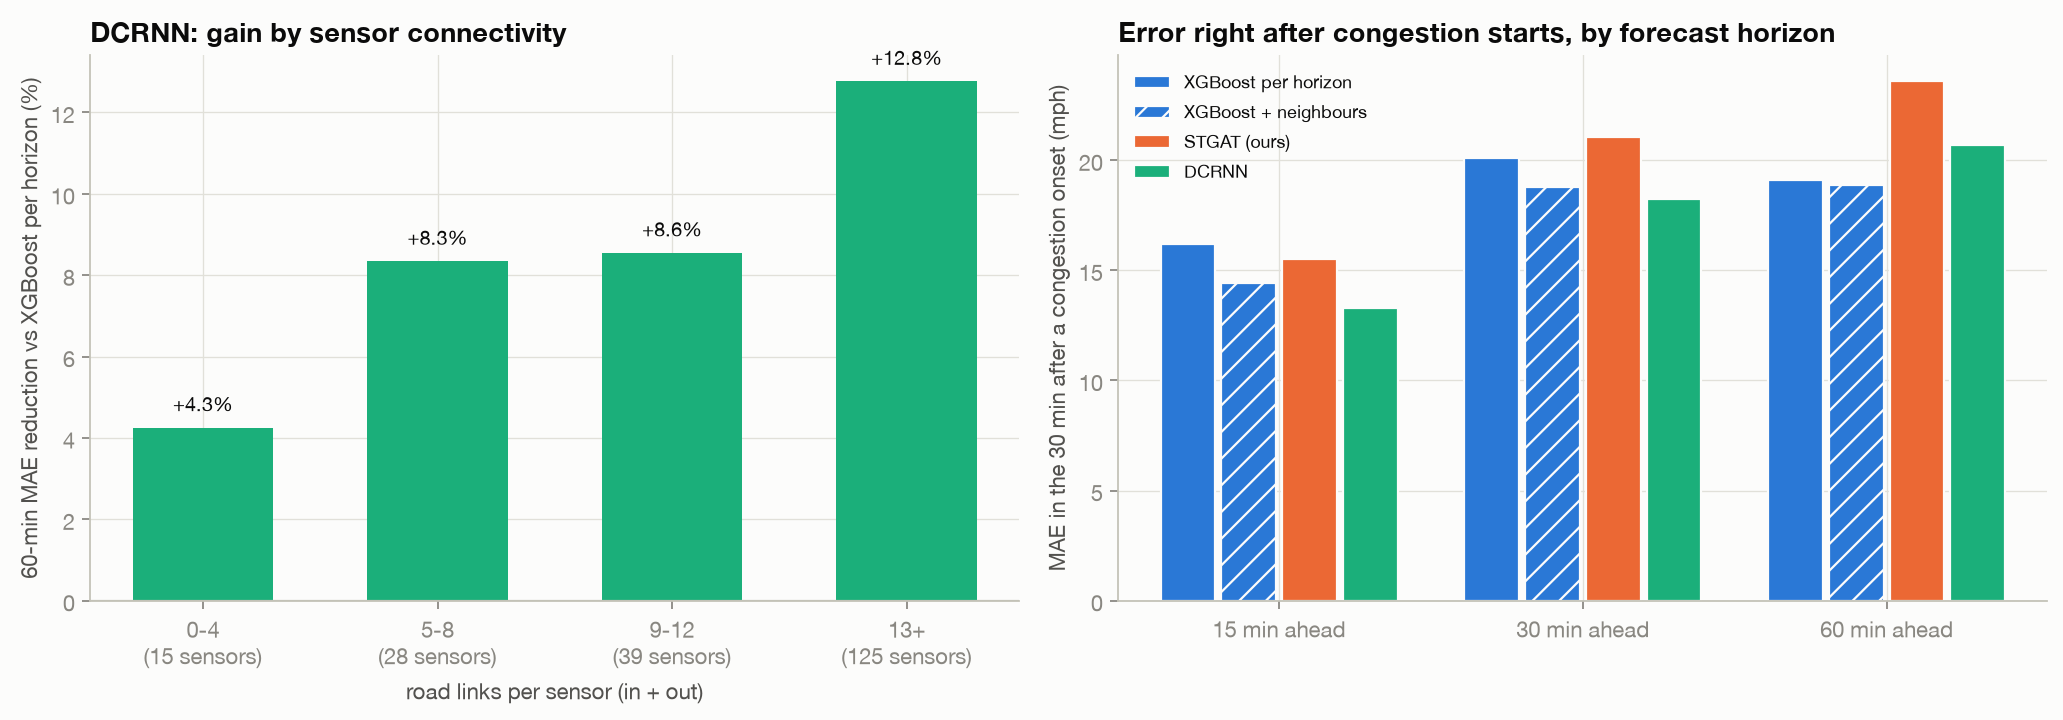
\includegraphics[width=0.49\textwidth]{fig17_where_the_graph_helps.png}\hfill
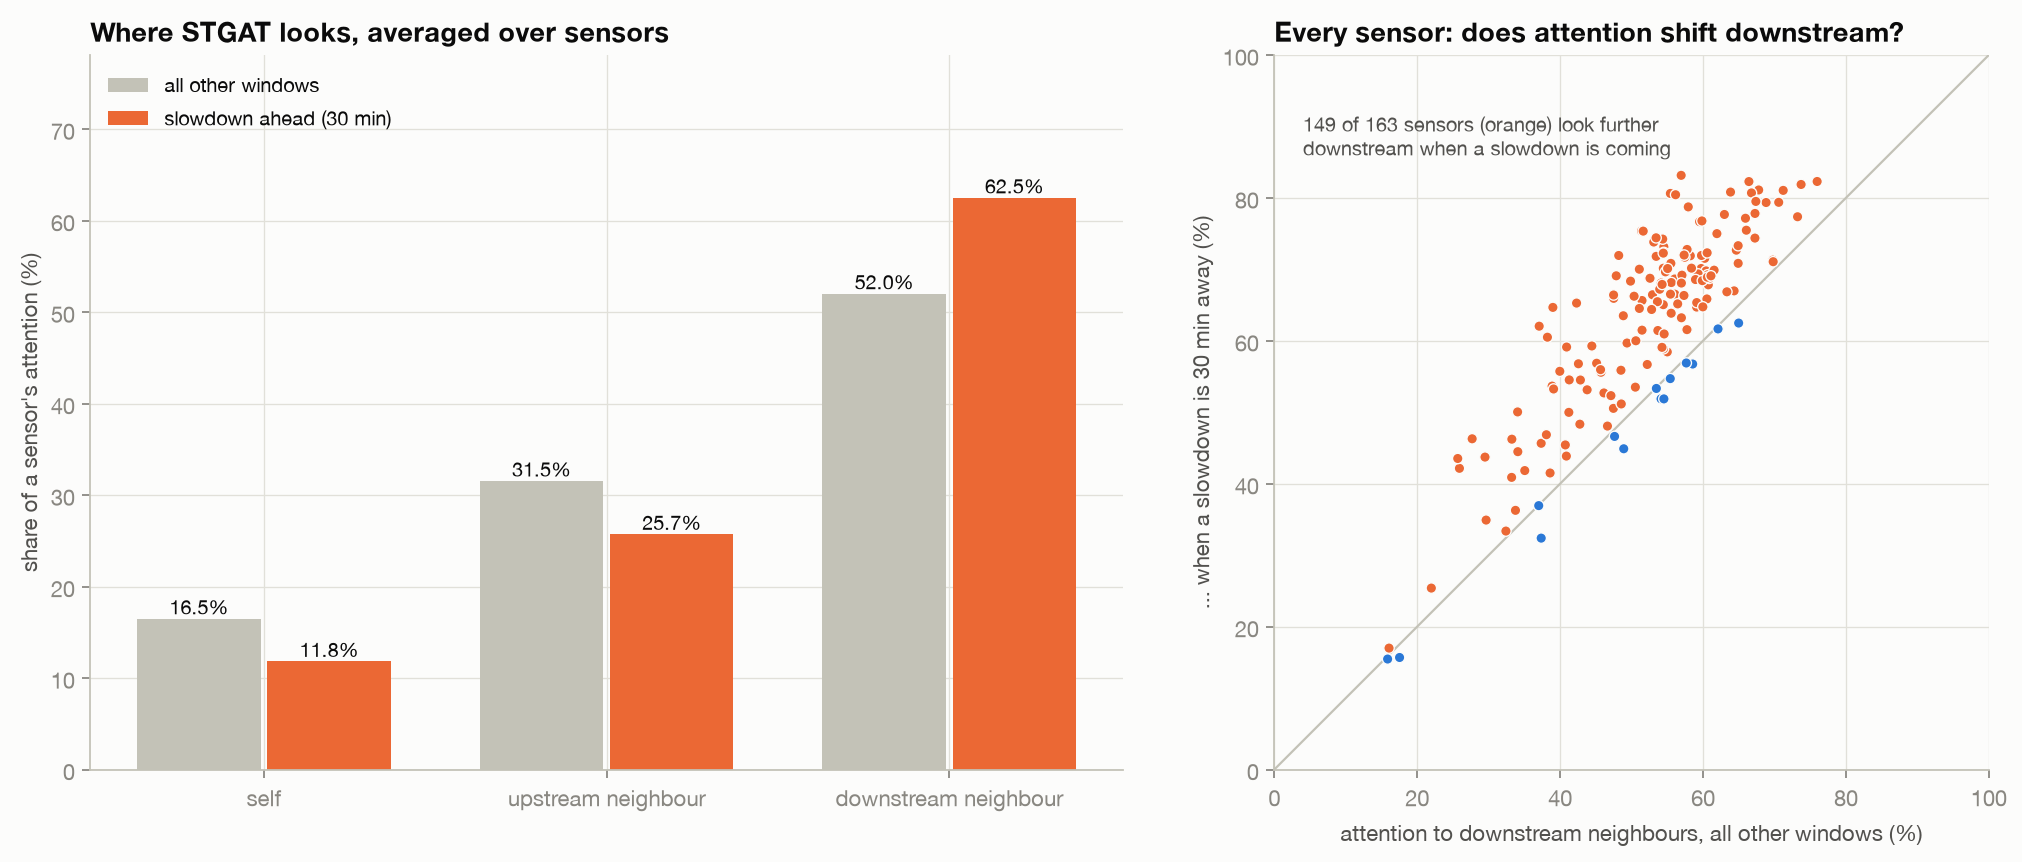
\includegraphics[width=0.49\textwidth]{fig14_attention.png}
\caption{Left: gain by sensor connectivity and error after congestion onsets. Right: STGAT attention by situation; when
a slowdown is 30 minutes away, attention moves to downstream neighbours.}
\label{fig:where}
\end{figure*}

\subsection{What the attention learned}
Averaged over \AttSensors{} sensors with both kinds of neighbours, STGAT gives \AttDownNormal\% of its attention to
downstream neighbours in normal windows and \AttDownAhead\% when the sensor will slow down within 30 minutes;
\AttShifted{} of the \AttSensors{} sensors shift downstream (Fig.~\ref{fig:where}). Nothing in the model says ``look
downstream''; it learned the direction that the data analysis found.

\subsection{Congestion maps}
At the busiest weekday PM-peak test moment (chosen by that rule, not by which model looks better), \MapCongested{} sensors
were congested; 30-minute forecasts caught \MapXgbCaught{} (XGBoost) and \MapGraphCaught{} (DCRNN). Over the test block,
DCRNN has the lower 60-minute error at \MapSensorsBetter{} of 207 sensors (Fig.~\ref{fig:map}).

\begin{figure*}[t]
\centering
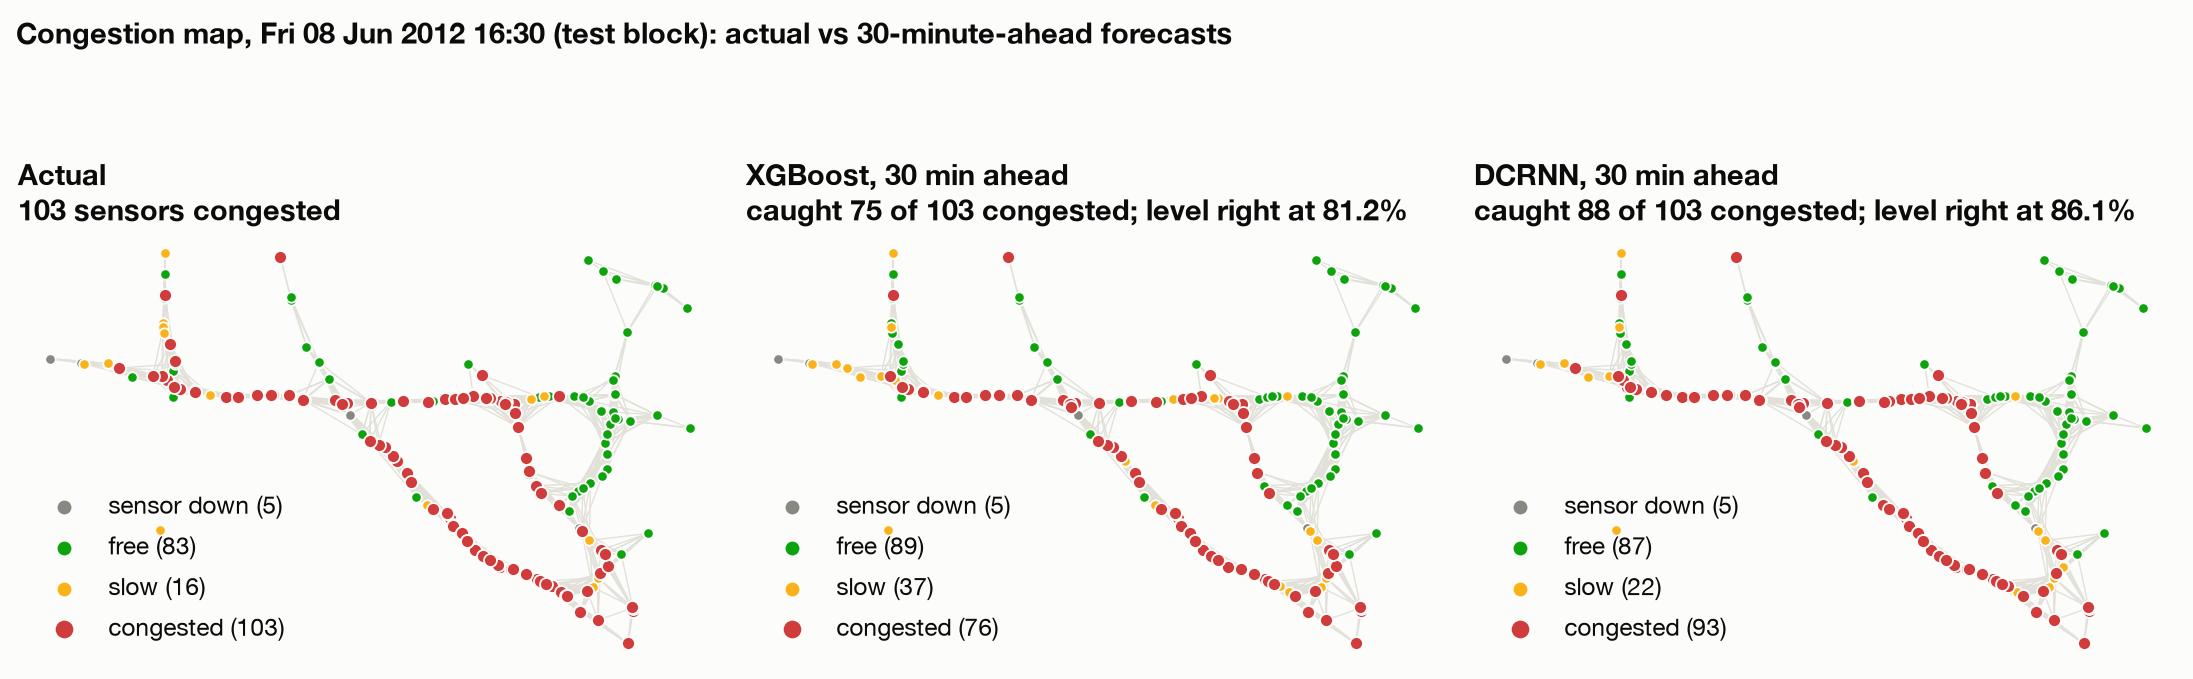
\includegraphics[width=0.82\textwidth]{fig18_congestion_map_side_by_side.png}
\caption{Congestion levels (speed over the sensor's free-flow speed) at a PM-peak test moment: actual, and 30-minute
forecasts by XGBoost and DCRNN.}
\label{fig:map}
\end{figure*}

\section{Discussion and Limitations}
Lower MAE does not mean fewer large misses: at 60 minutes DCRNN's RMSE is above XGBoost's, so a deployment that cares
about the worst errors should combine the two, which the hybrid does. Where the graph enters the model matters: DCRNN mixes neighbours at every recurrent step of encoding and decoding,
whereas STGAT mixes once after summarising each sensor; DCRNN's advantage persists at long horizons and STGAT's fades.
Limitations: METR-LA records speed only, so flow and occupancy features need PeMS data; the data cover one city's
freeways in 2012; ablations use one seed; the hybrid uses the validation block for fitting, which the per-sensor
baselines did not; and signal control is not evaluated: METR-LA freeways have no signals, and any control study would be
a simulation of a synthetic network, never live control.

\section{Conclusion}
Under a strict, shared protocol, graph neural networks close a real part of the spatial gap left by per-sensor models.
DCRNN improves on a tuned XGBoost by 11--13\% at every horizon and on every test day; the gain grows with sensor
connectivity, is largest right after congestion starts, and depends on the real road graph and on listening downstream.
A regularised tree corrector adds a further gain on top of the graph model, combining the graph's spatial view with the
trees' calendar knowledge.

\bibliographystyle{IEEEtran}
\bibliography{references}

\end{document}
